\section{What Lean verifies}
\label{sec:lean}

The proof problem has three interfaces. The metric calculation supplies a
specific projected forcing. The rational operator acts on a proposed row
of local coefficients. The retarded solution satisfies boundary
conditions on a physical exterior wave. Lean checks the implications
between these interfaces as well as the finite arithmetic at the
center of the exclusion.

\begin{figure}[htbp]
 \centering
 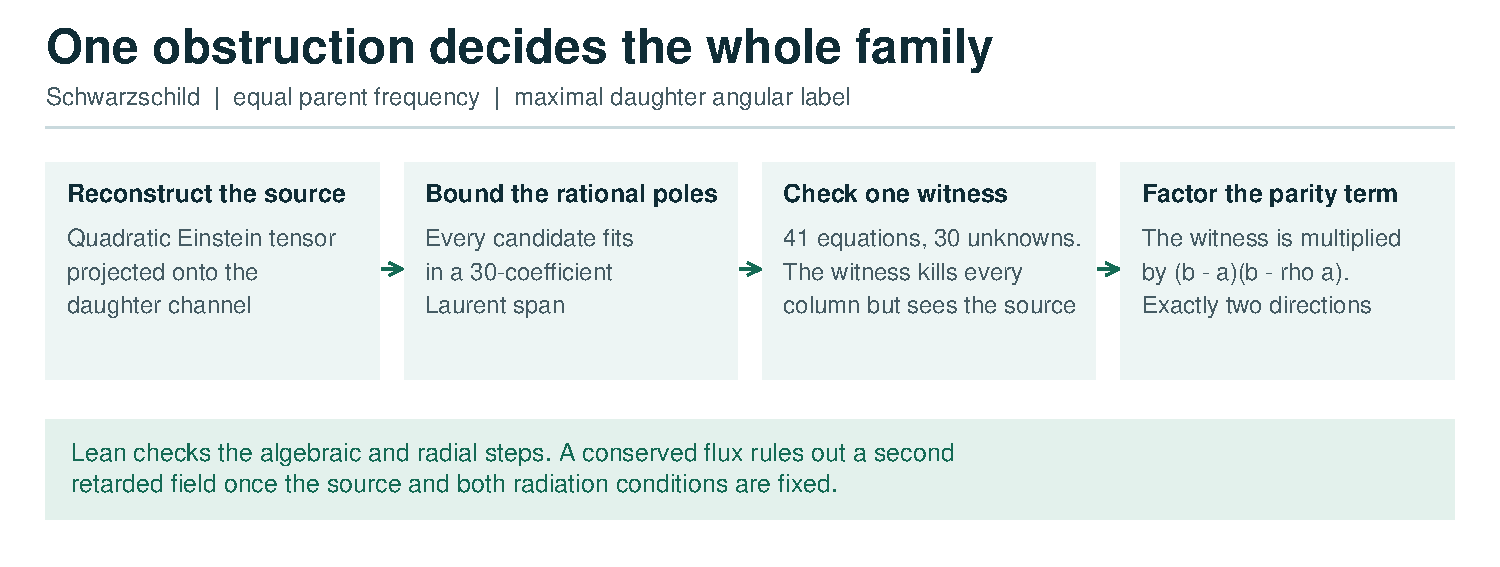
\includegraphics[width=\linewidth]{proof-chain.pdf}
 \caption{Structure of the classification argument. The 30 coefficients
 span all rational candidates after the pole and degree reductions.
 The witness is a linear functional of the 41 source equations. A
 nonzero witness projection proves that the source is outside the image
 of the operator.}
 \label{fig:proof-chain}
\end{figure}

\begin{description}
 \raggedright
 \item[Metric and source.] The checked coordinate and angular
 operations compute the quadratic Einstein tensor in the specified
 Schwarzschild perturbation ansatz. Separate reconstruction and
 conservation checks connect those components to the radial master
 source, including the relation to the pinned regularized source.
 \path{MetricMeromorphicClassification.lean} joins this chain to the
 local classification on a fixed nonzero parent germ.
 \item[All rational candidates.] The pole analysis at ordinary points,
 at the horizon and at zero, and the degree test at infinity reduce
 every possible row to the exhibited Laurent span.
 \path{MatrixCertificate.lean} checks the matrix columns and the
 source projection. The shifted coefficient sign proof covers every
 integer \(\ell\ge2\), and the exact parameter factors are nonzero at
 positive real frequency. The Riccati argument justifies coefficient
 matching even on a single parent solution.
 \item[Existence and uniqueness.] The checked source identities build
 a local row at each admitted ratio. \path{RationalLocalUniqueness.lean}
 rules out a nonzero rational homogeneous row.
 \path{LinearRetardedUniqueness.lean} proves the flux argument for the
 actual exterior boundary-value problem.
 \path{RetardedScattering.lean} constructs the two retarded fields and
 checks the printed strain formulas.
 \item[Extensions.]
 \path{AngularRetardedScattering.lean} proves existence and
 uniqueness for arbitrary azimuthal profiles in the top daughter.
 It combines two closed amplitudes with the pure-odd integral.
 Separate modules verify the angular obstruction, static comparison
 for the sharp-order absorption bound, the small-frequency magnitude
 sign calculation under the cited linear expansions, and the
 light-ring envelope transfer from its analytic matching hypotheses.
\end{description}

The guarded verification checked or hash-verified 1,208 modules in
the source and response development, with Lean 4.33.1 and a pinned
Mathlib revision. The named theorem checks require only the standard
Lean axioms \texttt{propext}, \texttt{Classical.choice} and
\texttt{Quot.sound}, or subsets. The public proof directory contains the
transitive source closure of the named results and lists the exact
toolchain and revision. It includes the algebraic polarization check
as a separately compiled extension.

Lean checks statements about the supplied equations and definitions.
The paper states the conventions that connect them to the physical
observables. The complex radial benchmarks and the fourth-multipole
zero enclosures use outward-rounded Arb arithmetic. The barrier-top
matching is an analytic argument, and the sign transfer explicitly
uses published linear expansion input. Related machine-checked
physics includes constructive field theory and local linear
Kerr--Newman perturbation equations \cite{douglas,wang}.
